\chapter{Konsistenz zwischen BPMN und BROS}
\label{chap:consistency}

Viele der bereits existierenden Verfahren lassen sich anpassen und können mit anderen Modellarten genutzt werden. 
Anstelle eines UML Klassendiagramms kann ein BROS Modell auf der strukturbasierten Seite und ein BPMN Modell anstelle eines UML-Sequenzdiagramms auf der verhaltensbasierten Seite verwendet werden.
Anders als bei UML ist bei dem Vergleich von BPMN und BROS zu beachten das Inkonsistenzen keine strikten Fehler, sondern nur Warnungen an den Modellierer sind.
Das liegt an dem Funktionsumfang von BROS Modellen.
Diese können gegenüber den BPMN Modellen, mit zusätzlich Elementen, angereichert werden.
So kann das BROS Modell zusätzliche Elemente beinhalten oder Teile des BPMN Modells auf einer höheren Ebene der Abstraktion darstellen.
Beispielsweise kann ein BROS-Event die Abstraktion eines gesamten Prozesses innerhalb des BPMN Modelles abbilden.
Um diese Konsistenzbeziehung genauer untersuchen zu können, muss zunächst geklärt werden, wie die Konsistenz zwischen Methoden definiert ist.
Dafür wird eine Definition des Konsistenzproblems gegeben
Anhand dieser werden verschiedene Regeln zur Konsistenzprüfung zwischen BPMN und BROS vorgestellt und ein Verfahren zur automatischen Prüfung dieser Regeln erläutert.

\section{Konsistenzproblem}

Wie bereits erwähnt, sind heutige Softwaresystem stark von den dazugehörigen Modellen abhängig.
Damit ein solches System erfolgreich implementiert werden kann müssen die Modelle konsistent zueinander sein.
Sollten schon zu Beginn eines Projektes unbemerkt Inkonsistenzen auftreten kann dies zum scheitern des gesamten Projektes führen.
Die verhaltensbasierten Modelle beschreiben die Interaktion innerhalb eines Systems.
Dabei benötigen sie die Funktionalität die von den strukturbasierten Modellen bereitgestellt wird.
Wenn sich die benötigte und die bereitgestellte Funktionalität unterscheidet kann das Softwaresystem nicht ordnungsgemäß funktionieren.
Solche Fehler stellen daher in der Industrie ein großes Risiko dar und können die Entwicklungskosten erheblich steigern.
Um dieses Risiko zu verringern müssen Verfahren entworfen werden, die ein möglichst automatisierte Konsistenzprüfung durchführen können.

Der methodische Entwicklung eines solchen Verfahrens setzt eine genaue Definition des Konsistenzproblems vorraus.
Allerdings ist eine formale und allgemeingültige Definition des Konsistenzproblem in der Domain der Modellierung in der Literatur nur schwer zu finden.
Bevor das Konsistenzproblem definiert werden kann muss zunächst beschieben werden was eine Inkonsistenz ist.
Laut \cite{Nuseibeh1996} tritt eine Inkonsistenz genau dann auf, wenn eine Konsistenzregel verletzt wird.
Eine Konsistenzregel ist eine Formalisierung von einem Aspekt der Konsistenz zwischen den betrachteten Modellen.
Dies kann in natürlicher Sprache oder in einer formalen Notation beschieben werden, wobei nur letzteres automatisiert überprüft werden kann.
Für die Definition nach \cite{Nuseibeh1996} wird das vorhandensein eines solchen Regelsatzes vorrausgesetzt.
Mit Hilfe dieser Definition kann das Konsistenzproblem wie folgt definiert werden:

\newtheorem*{konsistenzproblem}{Definition}

\begin{konsistenzproblem}
    Das Konsistenzproblem beschreibt den Vorgang der Minimierung und Verhinderung von Inkonsistenzen mit Hilfe der Aufstellung und Prüfung von Konsistenzregeln.
\end{konsistenzproblem}

Somit muss für die Entwicklung eines Konsistenzverfahrens zunächst definiert werden, welche Inkonsistenzen zwischen den Modellen existieren können und damit auf welchem Regelsatz das Verfahren basiert.
Anhand des aufgestellten Regelsatzes kann ein Algorithmus zum auffinden der Inkonsistenzen erstellt werden.
Dafür müssen die Regeln, wie bereits erwähnt, in einer formalen Form und nicht in natürlicher Sprache vorliegen.
Die Aufgabe der Minimierung und Verhinderung der Inkonsistenz ist auch mit einem automatisierten Tool dem Modellierer überlassen.
Die Verfahren können dem Modellierer Handlungsempfehlungen geben, eine automatische Korrektur ist allerdings nur schwer möglich.
So könnte ein Problem zB. durch das entfernen eines Elementes behoben werden, wodurch kaskadierend nochmehr Konsistenzfehler entstehen könnten.
Da diese Definition auf der Überprüfung von Regeln aufbaut, ist sie leicht auf Verfahren anwendbar, die für die Konsistenzprüfung, ebenfalls auf einem Regelsatz basieren.
Aber auch formale Verfahren ohne einen eigenen Regelsatz lassen sich mit dieser Definition beschreiben.
So können z.B. die Verfahren, die auf der Transformation zu einem Petrinetz basieren mittels der Konsistenzregel ``das konstruierte Petrinetz muss lebendig sein'' überprüft werden.

\section{Konsistenzregeln} \label{sec:Konsistenzregeln}

Das hier vorgestellte Verfahren basiert auf der \emph{Intra-Modell} bzw. horizontalen Konsistenzprüfung ohne Zwischendarstellung.
Regeln zum direkten vergleich der Modelle können in zwei verschiedene Richtungen definiert werden.
Eine Regel kann aufgrund eines Merkmales des ersten Modelles ein Merkmal im zweiten Modell fordern oder umgekehrt.
Damit basieren diese Regeln auf der logischen Implikation.
Um eine reflexive Regel zu erhalten (logische Äquivalenz) müssen zwei Regeln erstellt werden die sowohl die Hin- als auch die Rückrichtung abdecken.
Im Bezug auf den Vergleich von BPMN und BROS bedeutet das, eine Regel hat immer ein Ursprungs- und ein Zielmodell.
Da BROS beliebig erweitert werden kann, ist kein strikter Vergleich zwischen BPMN und BROS möglich.
Aus diesem Grund sind die meisten Regel aus der Sicht des BPMN-Modelles aufgestellt.

Wie bereits in \cref{chap:background} erläutert lassen sich die BPMN- und BROS-Modelle, aufgrund ihrer Metamodelle, in Form von Graphen darstellen.
Mit Hilfe des Graph-Logik-Isomorphismus können dies Graphen auch in Form von Logikprogrammen ausgedrückt werden.
Für die Spezifikation der Regeln wird im nachfolgenden eine auf Prolog basierende Notation genutzt.
Dies ermöglicht eine einfache und leicht verständliche Darstellung der Regeln ohne eine eigene domänenspezifische Sprache einführen zu müssen.
Als Grundlage für die Konsistenzregeln werden die in \cref{lst:definition_facts} und \cref{lst:definition_predicats} aufgestellten Fakten und Prädikate genutzt.

Die Faktenbasis besteht aus vier Bestandteilen und bildet die gesamte Modellstruktur ab.
Mit dem Fakt \emph{bpmn/2} und \emph{bros/2} werden die jeweiligen Modellelemente aufgelistet und gleichzeitig ihren jeweiligen Typen zugeordnet.
Der Fakt \emph{relation/3} bildet eine Relation zwischen zwei Modellelementen von Quelle nach Ziel ab und ordnet dieser Relation gleichzeitig einen Typ zu.
Durch \emph{parent/2} wird der hierarchische Aufbau der Modelle abgebildet.
Dabei ist zu beachten das jedes Element nur einen Parent haben darf.
Es gilt implizit \emph{check\_parent(X) :- parent(X, A), parent(X, B) -> A == B.}.
Damit wird sichergestellt das es sich bei den Graphen der BPMN- und BROS-Modelle um Bäume handelt.
Allgemein ist zu beachten das dies keine Zwischendarstellung ist und nur zur syntaktischen Definition der Regeln genutzt wird.
Da der Graph des BPMN-Modelles und der Graph des BROS-Modelles disjunkt sind muss keine weitere Trennung der \emph{relation/3} und \emph{parent/2} Fakten durchgeführt werden.

\begin{lstlisting}[language=Prolog, caption=Definitionen der Faktenbasis, label=lst:definition_facts]
% Definition aller BPMN Elemente mit ihrem zugehörigem Typ.
bpmn(Bpmn, Type).

% Definition aller BROS Elemente mit ihrem zugehörigem Typ.
bros(Bros, Type).

% Definition aller Relationen von Quelle nach Ziel mit Typ.
relation(Source, Target, Type).

% Definition der Modellstruktur per Eltern-Kind Beziehung.
parent(Child, Parent).
\end{lstlisting}

Zusätzlich werden noch zwei Hilfsprädikate definiert.
Das Prädikat \emph{transitive\_parent/2} bildet den transitiven Abschluss der \emph{parent/2} Relation.
Jedem Kind werden all seine transitiven Eltern zugeordnet.
Dies beinhaltet auch die Abbildung der Identität.
Das wichtigste Prädikat ist \emph{match/2}.
Es bildet das Matching der BPMN-Elemente zu den BROS-Elementen ab.
Dabei wird angenommen das ein Matching bereits existiert, wodurch es im weiteren auch als Orakelfunktion bezeichnet wird.
Ein Matching ist die Menge der bidirektionalen Zuordnungen von BPMN-Elementen auf die dazugehörigen BROS-Elemente. 

\begin{lstlisting}[language=Prolog, caption=Definitionen der weiterführenden Regeln, label=lst:definition_predicats]
% Transitiver Abschluss der Modellstruktur.
transitive_parent(Child, Parent) :- 
    Child == Parent.
transitive_parent(Child, Parent) :- 
    parent(Child, Parent).
transitive_parent(Child, Parent) :- 
    transitive_parent(Child, X), parent(X, Parent).

% Orakel für das Matching von Modellelementen.
match(Bpmn, Bros).
\end{lstlisting}

Mit der Hilfe dieser Prädikate können nun Regeln für die Konsistenz zwischen BPMN- und BROS-Modellen erstellt werden.
Dafür wird jede Regeln erläutert und an einem Minimalbeispiel visualisiert.
Die darauffolgende Formalisierung in Prolog dient als Referenz für die weitere Arbeit.

\textbf{Regel 1:} 
Zu jedem \emph{BPMN-Process} muss eine \emph{BROS-Scene} oder ein \emph{BROS-Event} existieren.
Ein BPMN-Process stellt eine Umgebung für einen natürlichen Prozess dar.
In BROS wird dies mit einer BROS-Scene repräsentiert.
Allerdings kann ein BROS-Modell eine Abstraktion eines BPMN-Modelles sein.
In diesen Fall kann der BPMN-Process auch durch ein BROS-Event modelliert werden.
Durch diese Abstraktion muss der Inhalt des BPMN-Processes nicht weiter überprüft werden.
Dies ist exemplarisch in \cref{fig:ruleExample1} für eine BROS-Scene dargestellt.
In beiden Modellen muss der Prozess enthalten sein, der Inhalt und die Relationen werden nicht betrachtet.

\begin{lstlisting}[language=Prolog, caption=Formalisierung der Regel 1, label=lst:rule_1]
rule_1(Bpmn) :- bpmn(Bpmn, "Process") ->
    (
        bros(Bros, "Scene"), match(Bpmn, Bros);
        bros(Bros, "Event"), match(Bpmn, Bros)
    ).
\end{lstlisting}

\textbf{Regel 2:}
Zu jeder \emph{BPMN-Swimlane} innerhalb eines \emph{BPMN-Process} muss ein passender \emph{BROS-RoleType} existieren.
Eine Swimlane stellt einen Teilnehmer innerhalb des BPMN-Prozesses dar. 
Dieses Konzept wird in BROS mittels Rollen dargestellt.
Daher muss jeder Teilnehmer des BPMN-Prozesses auch als Rolle im BROS-Modell existieren.
In \cref{fig:ruleExample2} existiert in dem BPMN-Modell eine BPMN-Swimlane ''Kunde'', welche im BROS-Modell als BROS-RoleType ''Kunde'' dargestellt wird.

\begin{lstlisting}[language=Prolog, caption=Formalisierung der Regel 2, label=lst:rule_2]
rule_2(Bpmn) :- bpmn(Bpmn, "Swimlane") ->
    (
        bros(Bros, "RoleType"), match(Bpmn, Bros)
    ).
\end{lstlisting}

\textbf{Regel 3:}
Zu jedem \emph{BPMN-TerminationEvent} muss eine \emph{BROS-ReturnEvent} existieren.
Eine BPMN-TerminationEvent beendet den aktuellen BPMN-Prozess.
Der BPMN-Prozess wird in BROS durch eine BROS-Scene dargestellt (vgl. \textbf{Regel 1}).
Eine BROS-Scene wird durch ein BROS-ReturnEvent beendet.
Somit muss ein BPMN-TerminationEvent mit einem BROS-ReturnEvent modelliert werden.
Diese Regel wird in \cref{fig:ruleExample3} visualisiert.

\begin{lstlisting}[language=Prolog, caption=Formalisierung der Regel 3, label=lst:rule_3]
rule_3(Bpmn) :- bpmn(Bpmn, "TerminationEvent") ->
    (
        bros(Bros, "ReturnEvent"), 
        match(Bpmn, Bros),
        (
            parent(Bros, BrosParent),
            transitive_parent(Bpmn, BpmnParent),
            match(BpmnParent, BrosParent)
        )
    ).
\end{lstlisting}

\textbf{Regel 4:}
Zu jedem \emph{BPMN-EndEvent} muss ein \emph{BROS-Event} oder \emph{BROS-ReturnEvent} existieren.
Ein BPMN-EndEvent beendet die aktuelle BPMN-Swimlane.
Jede BPMN-Swimlane wird von einem BROS-RoleType repräsentiert (Vgl. \textbf{Regel 2}).
Ein BROS-RoleType wird mit einem BROS-Event beendet, wenn zwischen diesen beiden eine BROS-DestroyRelation existiert.
Alternativ kann ein BPMN-EndEvent auch durch ein BROS-ReturnEvent modelliert werden, wenn das BPMN-EndEvent das abschließende Event des BPMN-Prozesses ist.
Der erste Fall ist mit Hilfe des Prozessteilnehmers ''Kunde'' in \cref{fig:ruleExample4} beispielhaft dargestellt.

\begin{lstlisting}[language=Prolog, caption=Formalisierung der Regel 4, label=lst:rule_4]
rule_4(Bpmn) :- bpmn(Bpmn, "EndEvent") ->
    (
        (
            bros(Bros, "Event"),
            match(Bpmn, Bros),
            (
                relation(RoleType, Bros, "DestroyRelation"),
                transitive_parent(Bpmn, BpmnParent),
                match(BpmnParent, RoleType)
            )
        );
        (
            bros(Bros, "ReturnEvent"), 
            match(Bpmn, Bros),
            (
                parent(Bros, BrosParent),
                transitive_parent(Bpmn, BpmnParent),
                match(BpmnParent, BrosParent)
            )
        )
    ).
\end{lstlisting}

\textbf{Regel 5:}
Zu jedem \emph{BPMN-StartEvent} muss ein \emph{BROS-Event} existieren.
Ein BPMN-StartEvent beginnt die aktuelle BPMN-Swimlane.
Jede BPMN-Swimlane wird von einem BROS-RoleType repräsentiert (vgl. \textbf{Regel 2}).
Ein BROS-RoleType wird mit einem BROS-Event begonnen, wenn  zwischen diesen beiden eine BROS-CreateRelation existiert.
Alternativ kann ein BPMN-StartEvent auch durch ein BROS-Event modelliert werden, wenn das BPMN-StartEvent das erste Event des BPMN-Prozesses ist und eine BROS-CreateRelation zwischen dem BROS-Event und der BROS-Scene existiert, die den BROS-Prozess darstellt (vgl. \textbf{Regel 1}).
Diese Regel entspricht, im Sinne des Ablaufes des Geschäftsprozesses, dem Gegenstück zu \textbf{Regel 4}.
Die Visualisierung nutzt das gleiche Beispiel, nur ist in \cref{fig:ruleExample5} der Fokus auf das BPMN-StartEvent und die BROS-CreateRelation gelegt.

\begin{lstlisting}[language=Prolog, caption=Formalisierung der Regel 5, label=lst:rule_5]
rule_5(Bpmn) :- bpmn(Bpmn, "StartEvent") ->
    (
        bros(Bros, "Event"),
        match(Bpmn, Bros),
        (
            relation(Bros, X, "CreateRelation"),
            transitive_parent(Bpmn, BpmnParent),
            match(BpmnParent, X)
        )
    ).
\end{lstlisting}

\textbf{Regel 6:}
Zu jedem \emph{BROS-Event} bzw. \emph{BROS-ReturnEvent} muss ein \emph{BPMN-Element} existieren.
Dies ist die einzige Regel die von dem BROS-Modell aus das BPMN-Modell überprüft.
Jedes \emph{BROS-Event} bzw. \emph{BROS-ReturnEvent} muss eine Ursache im BPMN-Modell haben.
Es darf kein Event im BROS-Modell geben das nicht im BPMN-Prozess existiert.
Ein solches BROS-Event hätte keinen Auslöser im Verhaltensmodell und könnte somit nie eintreten.
Passende BPMN-Elemente sind BPMN-Events unabhängig vom Typ, BPMN-Activities oder auch Ausgänge eines BPMN-Gateways.
beispielhaft ist diese Regel in \cref{fig:ruleExample6} dargestellt.
Hier wird der Fall abgebildet, das ein BROS-Event mit einem BPMN-Gateway übereinstimmt.

\begin{lstlisting}[language=Prolog, caption=Formalisierung der Regel 6, label=lst:rule_6]
rule_6(Bros) :- (bros(Bros, "Event"); bros(Bros, "ReturnEvent")) ->
    (
        bpmn(Bpmn, "StartEvent"), match(Bpmn, Bros);
        bpmn(Bpmn, "EndEvent"), match(Bpmn, Bros);
        bpmn(Bpmn, "TerminationEvent"), match(Bpmn, Bros);
        bpmn(Bpmn, "Event"), match(Bpmn, Bros);
        bpmn(Bpmn, "Activity"), match(Bpmn, Bros);
        bpmn(Bpmn, "Gateway"), match(Bpmn, Bros)
    ).
\end{lstlisting}

\begin{figure}
    \centering
    \begin{subfigure}{0.4\textwidth}
        \centering
        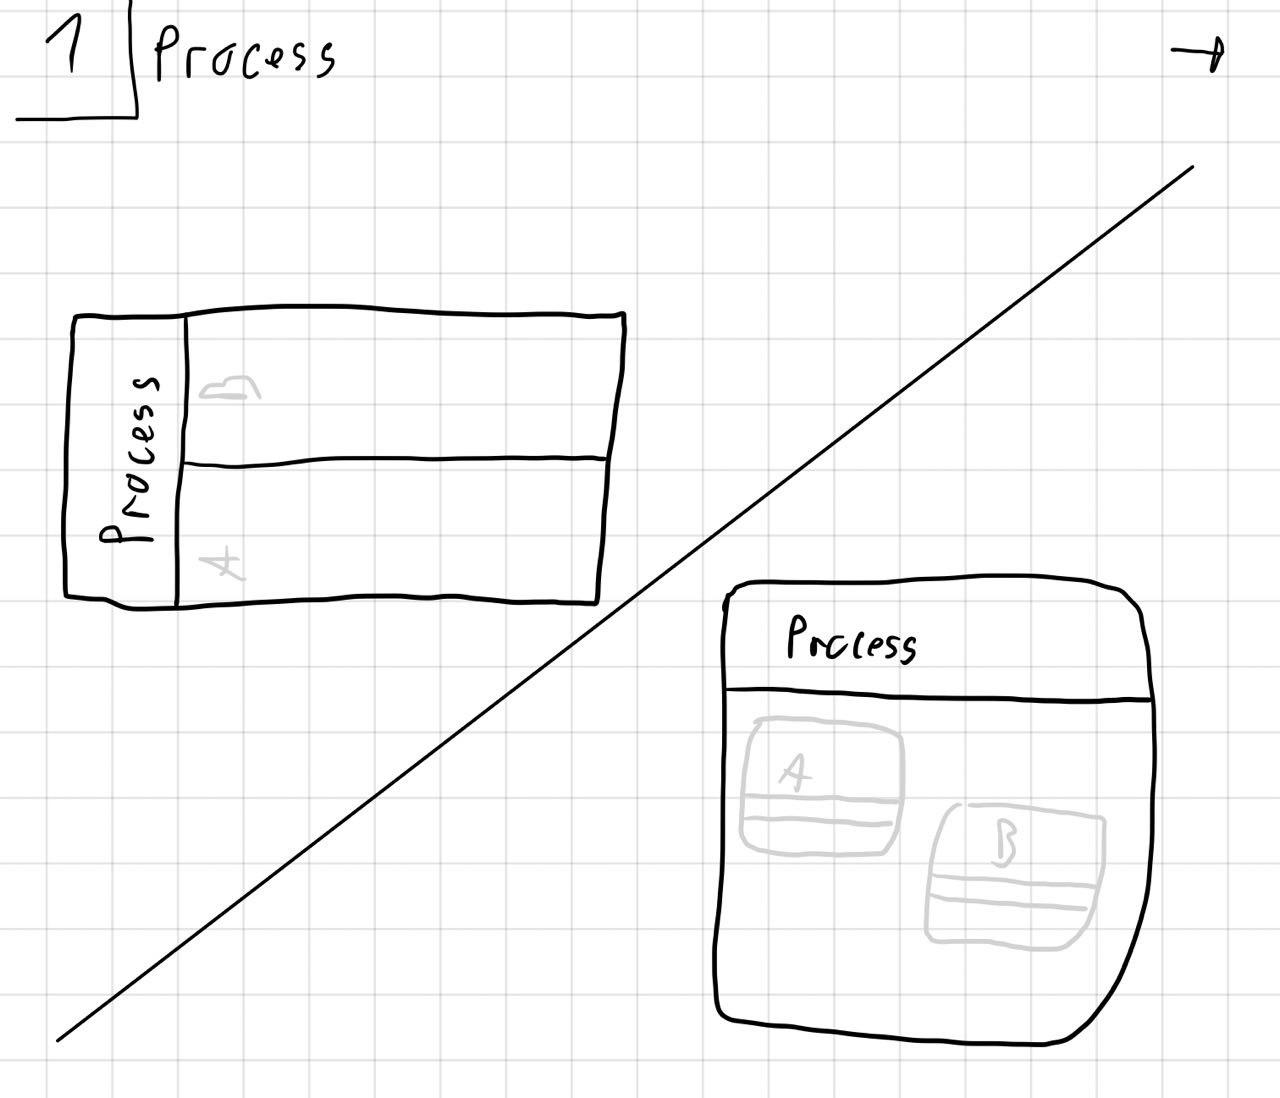
\includegraphics[width=\textwidth,keepaspectratio]{../images/rule/rule1.jpg}%
        \caption{Darstellungen der Regel 1}%
        \label{fig:ruleExample1}
    \end{subfigure}
    \hfill
    \begin{subfigure}{0.4\textwidth}
        \centering
        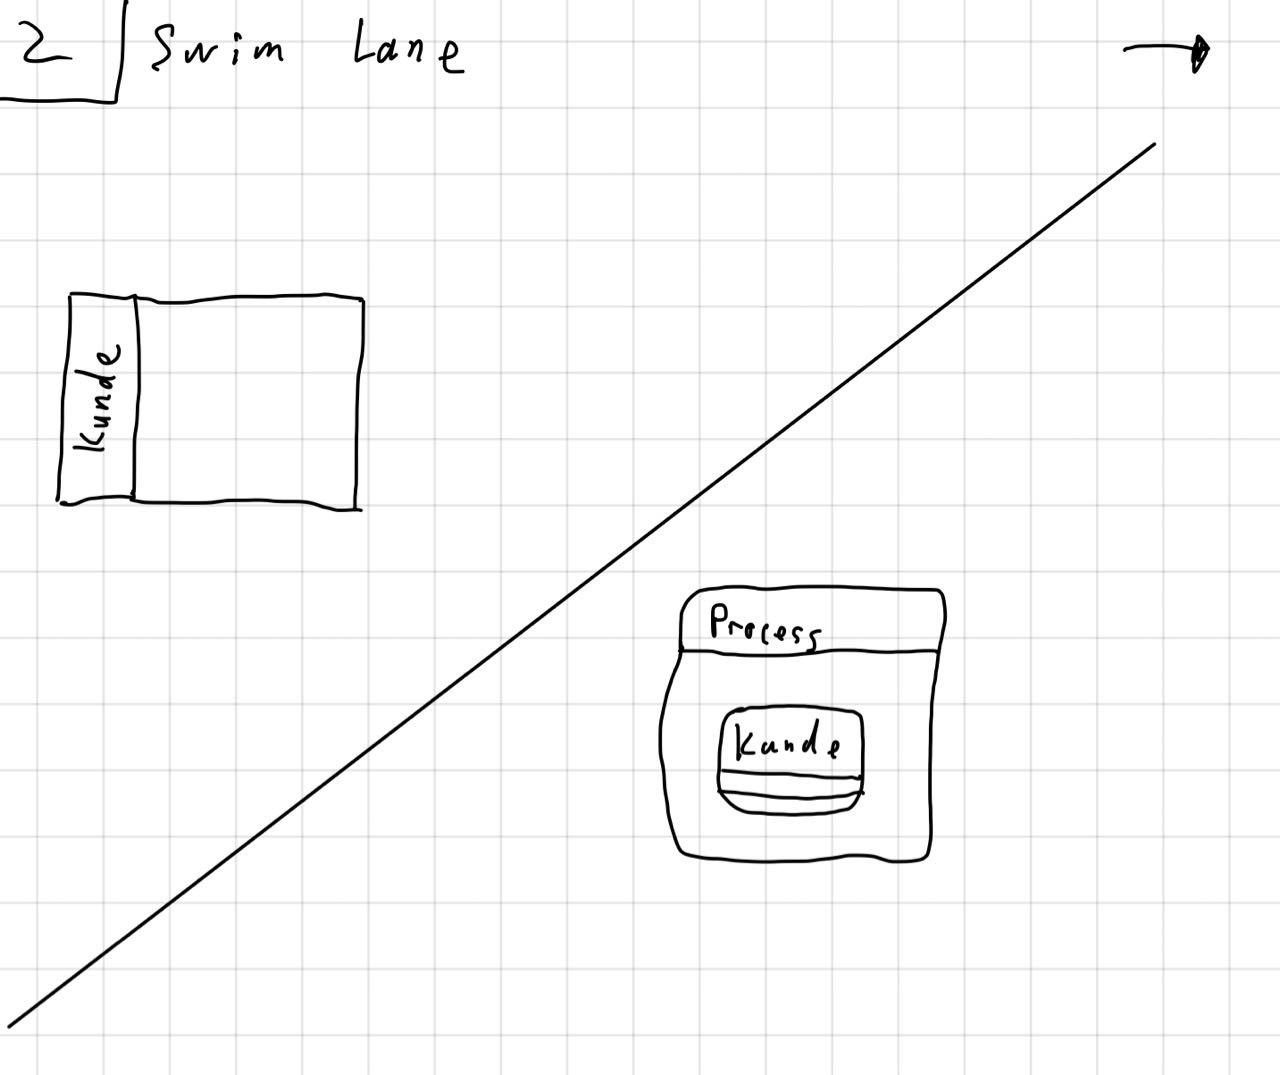
\includegraphics[width=\textwidth,keepaspectratio]{../images/rule/rule2.jpg}%
        \caption{Darstellungen der Regel 2}%
        \label{fig:ruleExample2}
    \end{subfigure}
    \begin{subfigure}{0.4\textwidth}
        \vspace{20pt}
        \centering
        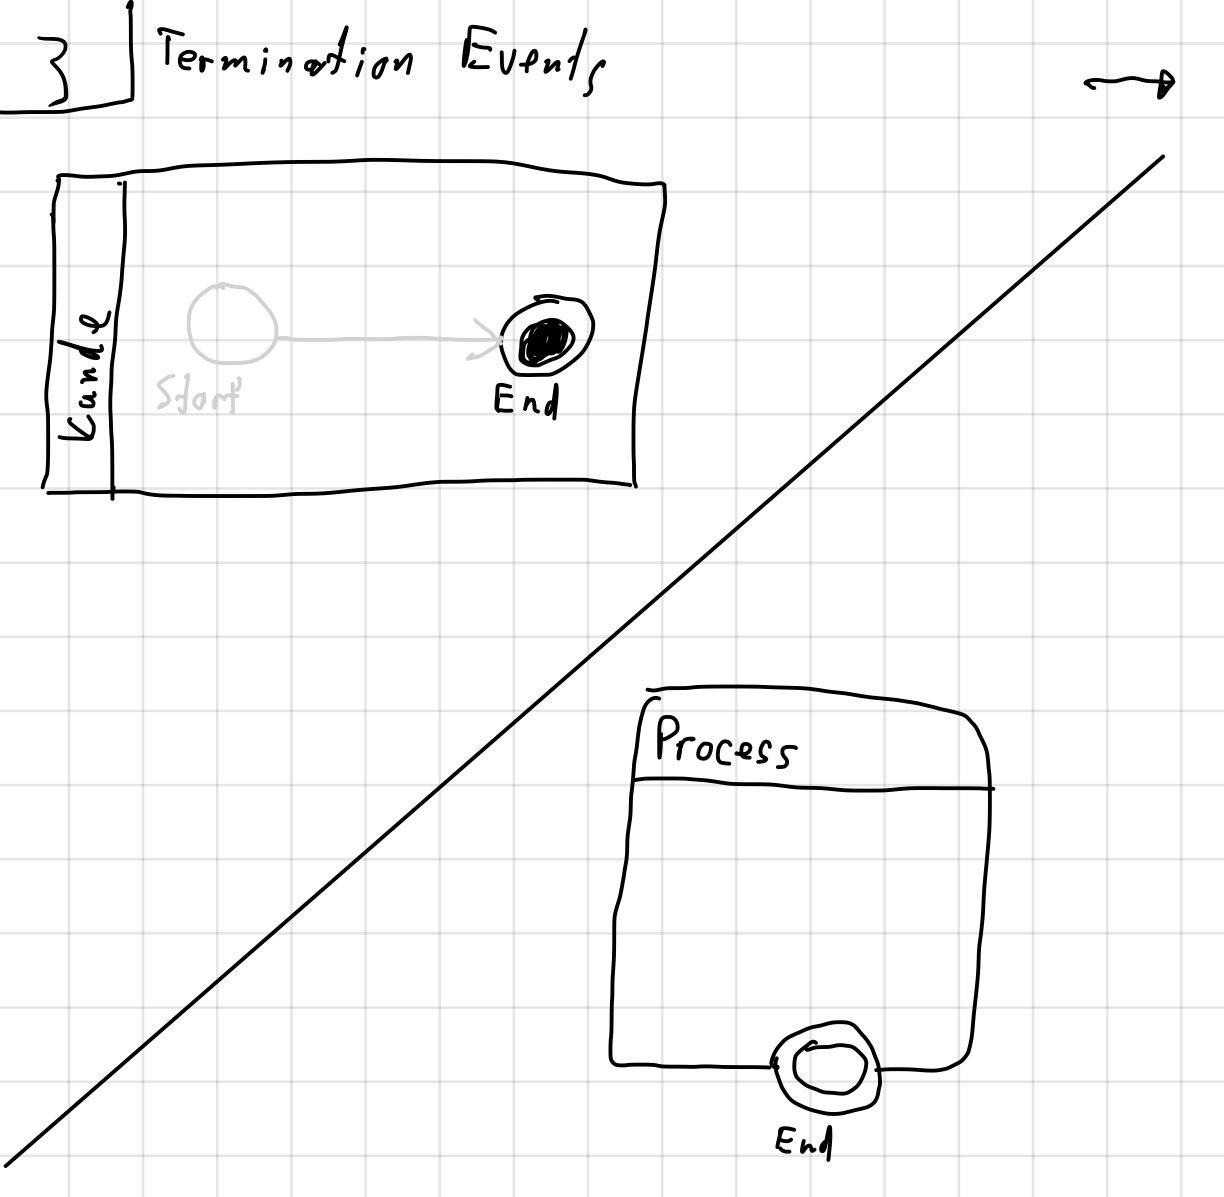
\includegraphics[width=\textwidth,keepaspectratio]{../images/rule/rule3.jpg}%
        \caption{Darstellungen der Regel 3}%
        \label{fig:ruleExample3}
    \end{subfigure}
    \hfill
    \begin{subfigure}{0.4\textwidth}
        \vspace{20pt}
        \centering
        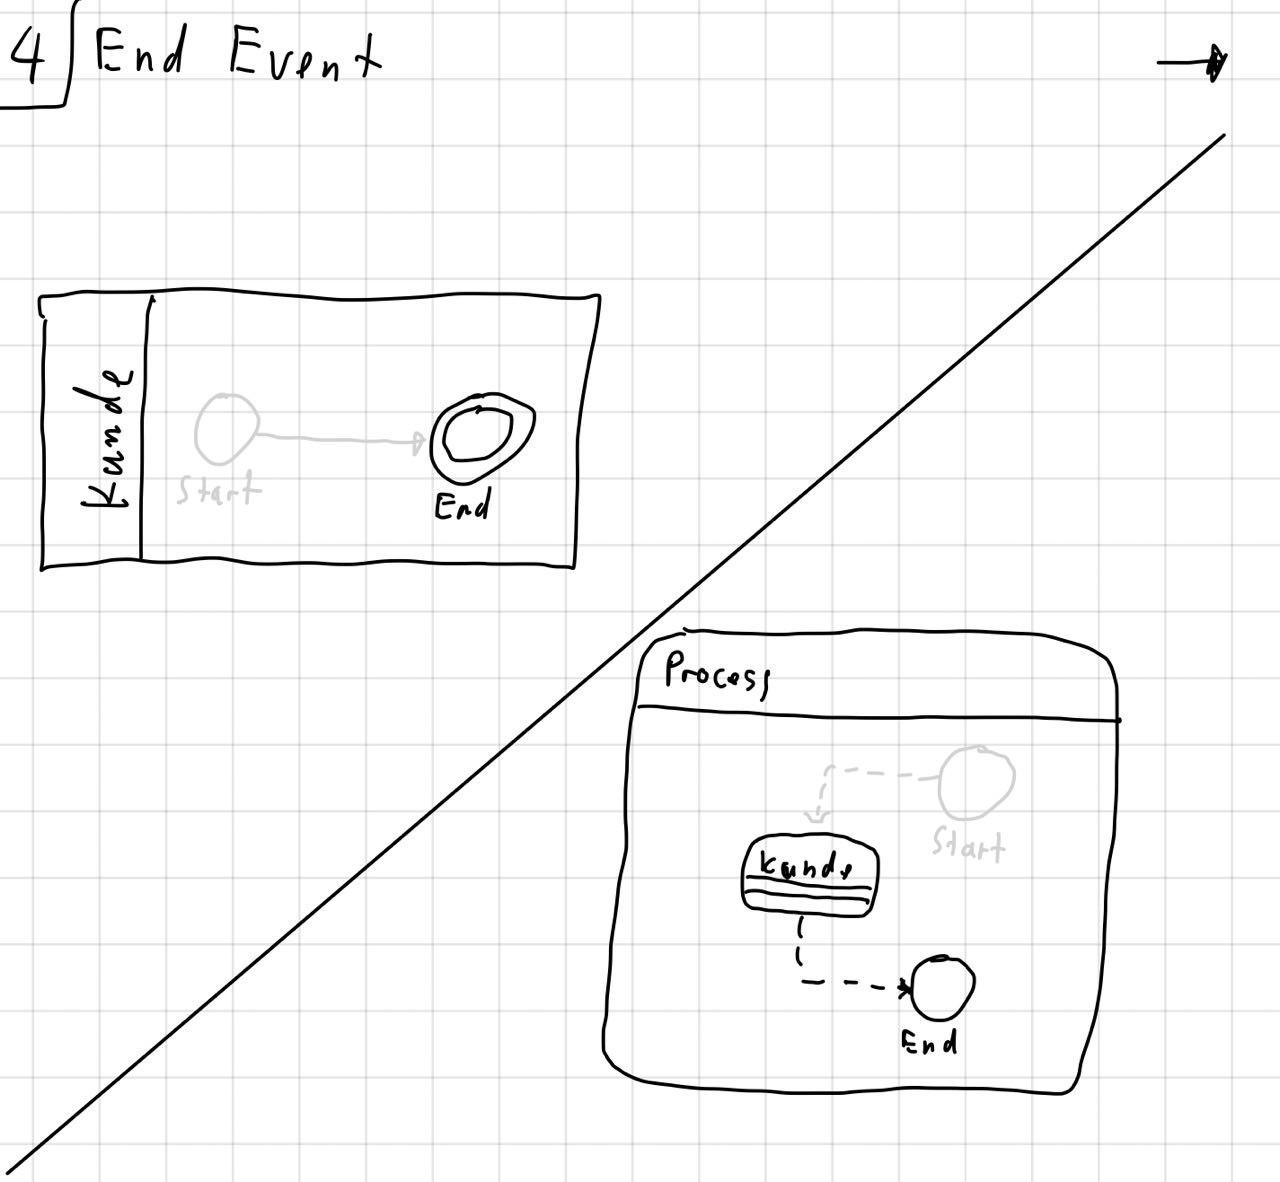
\includegraphics[width=\textwidth,keepaspectratio]{../images/rule/rule4.jpg}%
        \caption{Darstellungen der Regel 4}%
        \label{fig:ruleExample4}
    \end{subfigure}
    \begin{subfigure}{0.4\textwidth}
        \vspace{20pt}
        \centering
        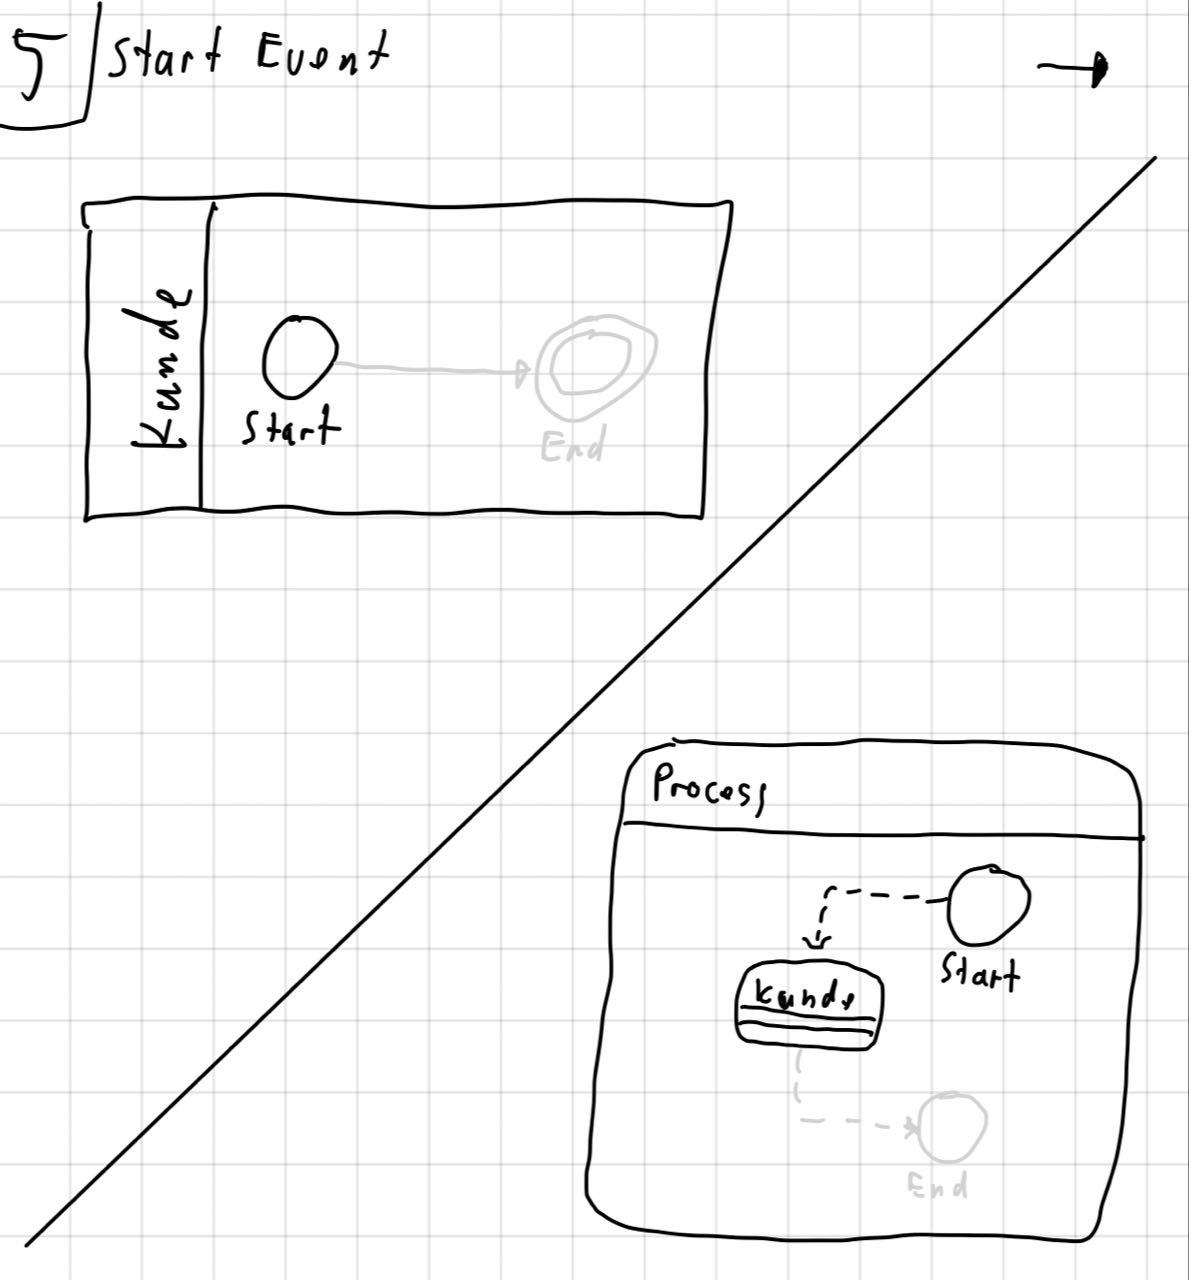
\includegraphics[width=\textwidth,keepaspectratio]{../images/rule/rule5.jpg}%
        \caption{Darstellungen der Regel 5}%
        \label{fig:ruleExample5}
    \end{subfigure}
    \hfill
    \begin{subfigure}{0.4\textwidth}
        \vspace{20pt}
        \centering
        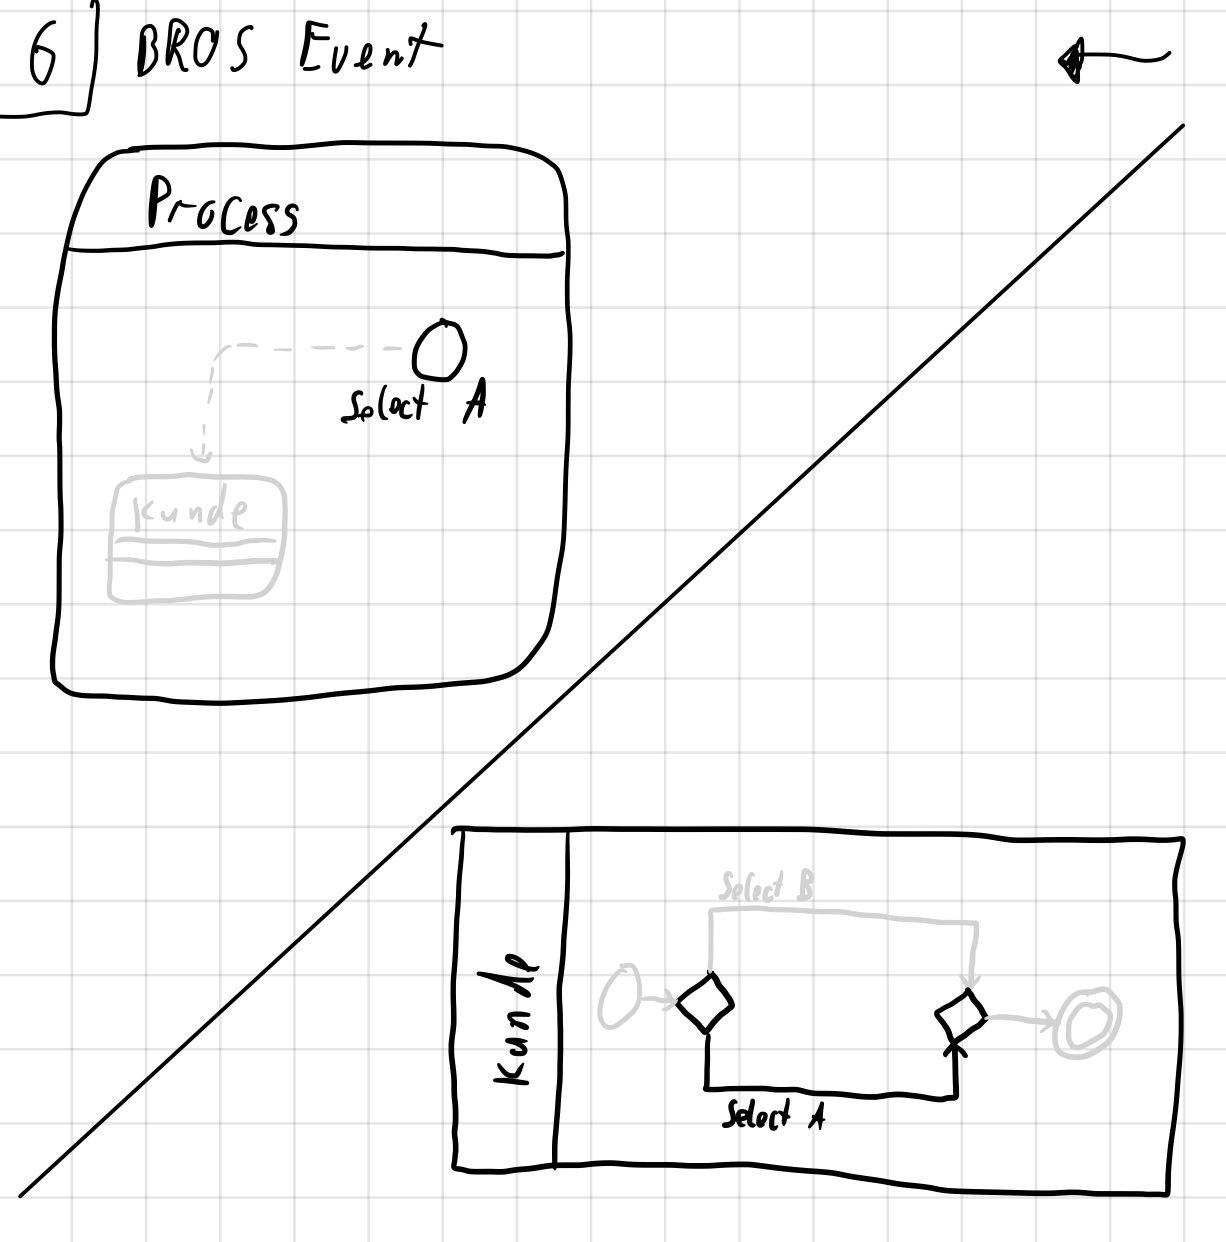
\includegraphics[width=\textwidth,keepaspectratio]{../images/rule/rule6.jpg}%
        \caption{Darstellungen der Regel 6}%
        \label{fig:ruleExample6}
    \end{subfigure}
    \caption{Exemplarische Darstellungen der Konsistenzregeln 1-6}%
    \label{fig:pizzaBrosSteps}
\end{figure}

\section{Referenzarchitektur}

Im Gegensatz zu anderen Arbeiten wurde zur Überprüfung dieser Regeln kein formales Verfahren auf Basis von z.B. \emph{Description Logic} oder \emph{Petrinetzen} genutzt.
Dies hat den Vorteil das die Regeln direkt auf den Modellen ausgeführt werden können und nicht erst eine Zwischendarstellung konstruiert werden muss.
Das hier genutzte Verfahren arbeitet in zwei Stufen auf den Modellen, die als geschichteter Graph dargestellt werden.
Im ersten Schritt wird ein Matching von Modellelementen aufgebaut.
Dies wird iterativ, in Form eines Fixpunkt-Algorithmus, durchgeführt um kaskadierendes Matching zu erlauben.
Dieser Schritt wird im folgenden \emph{Matching-Algorithmus} genannt.
Im zweiten Schritt werden anhand dem Matching die erstellten Regeln ausgeführt.
Dabei werden die Regelergebnisse aggregiert.
Dieser Vorgang wird als \emph{Verifikations-Algorithmus} bezeichnet.

\begin{figure}
    \centering
    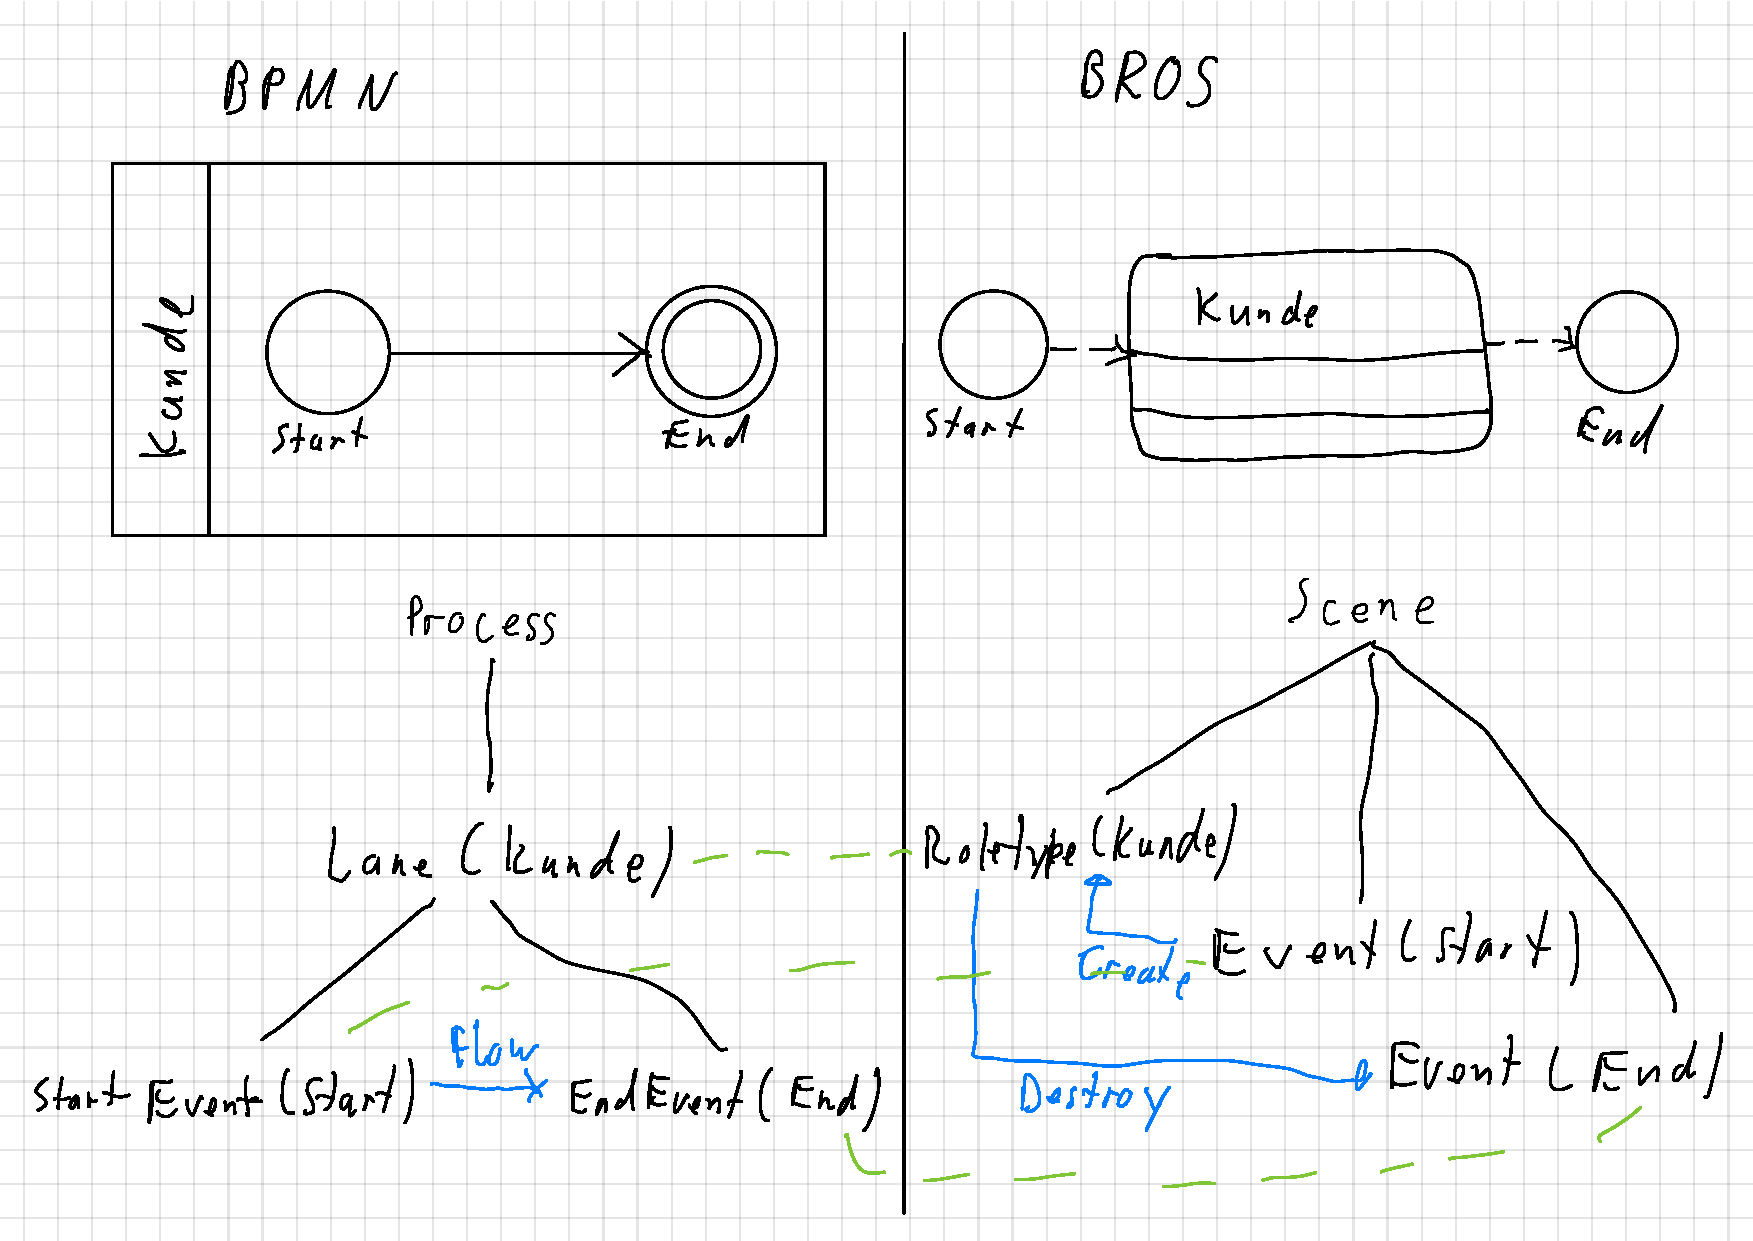
\includegraphics[width=\textwidth,keepaspectratio]{../images/ModelToGraph.pdf}%
    \caption{Visualisierung des Graph Matching}%
    \label{fig:ModelToGraph}
\end{figure}

Um das Verfahren anzuwenden, müssen beiden Modelle in Form eines gerichteten Graph vorliegen, der aus mehreren Ebenen besteht.
Ein geschichteter Graph basiert auf einem Baum der die Grundstruktur des Modelles und die Eltern-Kind Beziehung abdeckt.
Um die Relationen zwischen den Modellelementen darzustellen wird ein Schicht mit Querverweisen über den Baum gelegt.
In \cref{fig:ModelToGraph} wird die Transformation der Modelle in die dazugehörigen Graphen dargestellt.
Auf der linken Seite ist ein BPMN-Modell mit dem dazugehörigen Graphen. 
Auf der rechten Seite ist ein vereinfachtes BROS-Modell mit seinem Graphen.
Der schwarze Teil der Graphen bildet die Grundstruktur oder auch die erste Schicht.
Dieser wird mit Hilfe der ``contains''-Relation der Metamodelle direkt aufgebaut.
In blau ist die zweite Schicht, die Schicht der Relationen, visualisiert.
Jede Relation ist mit ihrem Typ annotiert und hat eine feste Richtung.
Die Graphen des BPMN-Modelles und des BROS-Modelles sind zueinander disjunkt.

Mit beiden Graphen kann nun der Matching-Algorithmus durchgeführt werden.
Das Matching ist die dritte Schicht innerhalb der Graphen, die den Graphen des BPMN-Modelles mit dem Graphen des BROS-Modelles verbindet.
In \cref{fig:ModelToGraph} wird dies in grün dargestellt.
Um diese Schicht zu konstruieren wird eine Orakelfunktion genutzt.
Diese ermittelt ob zwei Elemente zueinander passend sind.
Dabei hat die Orakelfunktion zwei Parameter, den aktuellen Konten des BPMN-Graphen und den des BROS-Graphen.
Die übergebenen Knoten enthalten Referenzen auf ihre Relationen aus allen drei Schichten.
In der ersten Schicht sind die Vorfahren und Nachkommen und in der zweiten Schicht die per Relation verbunden Elemente.
Die dritte Schicht ist zu Beginn leer.
Wenn die Orakelfunktion für das BPMN-Element \emph{x} und das BROS-Element \emph{y} ein Matching feststellt, werden die Kanten \emph{(x, y)} und \emph{(y, x)} der dritten Schicht hinzugefügt.
Eine einmal hinzugefügt Kante kann nicht wieder entfernt werden.
Da die dritte Schicht auch mit an das Orakel übergeben wird, kann dieses aufgrund von einem bereits bestehen Matching eine Entscheidung treffen.
Um dieses Verhalten zu nutzen wird der Vorgang des Matchingaufbaues solange wiederholt bis sich die dritte Schicht nicht weiter ändert.
Dieses Verhalten wird Fixpunkt-Algorithmus genannt.
Innerhalb einer Iteration des Algorithmus wird die Orakelfunktion auf allen Paaren von Elementen des BPMN- und des BROS-Modelles angewendet.
Ein Fixpunkt-Algorithmus kann unter umständen nicht terminieren, wenn die Datenstruktur in eine oszillierenden Zustand übergeht.
Dies wird verhindert indem Kanten nur zu dem Matching hinzugefügen werden und somit nie entfernt werden dürfen, wodurch das Matching monoton wachsend ist.
Damit kann die dritte Schicht maximal zu einem vollständigen Graphen anwachsen.
Anschließend kann keine weitere Kante hinzugefügt werden und der Algorithmus terminiert automatisch.

Mit dem konstruierten Matching kann nun der Verifikations-Algorithmus ausgeführt werden.
In diesem Schritt werden die unter \cref{sec:Konsistenzregeln} aufgestellten Konsistenzregeln überprüft.
Diese Überprüfung kann mittels der genannten Prolog Regeln oder auch direkt auf den Graphen durchgeführt werden.
Anders als der Matching-Algorithmus wird der Verifikations-Algorithmus nur einmal durchlaufen.
Da alle Regeln die Konsistenzprüfung von einem Modell auf das andere Modell durchführen, können die Regeln die auf dem BPMN-Modell basieren unabhängig von den Regeln die auf dem BROS-Modell basieren ausgeführt werden.
So werden die Regeln die die Überprüfung aus Sicht des BPMN-Modelles ausführen, für jedes Element des BPMN-Graphen angewendet.
Um eine bessere Fehlermeldung für den Modellierer zu erstellen, wird im Falle einer Regelverletzung nicht nur das BPMN-Element, sondern auch das BROS-Element das zu dem Regelverstoß führt, als negative Konsistenzmeldung gespeichert.
Mit Hilfe der beiden Elemente und der verletzen Regel kann eine genaue Fehlerbeschreibung gegeben werden.
Dieses Verhalten ist analog für die Regel die aus Sicht des BROS-Modelles arbeiten.
Nicht mit den Prologregeln dargestellbar ist der Unterschied zwischen erfolgreichen und abgebrochenen Regelprüfungen.
Jede Regel hat zu beginn eine Implikation, die die Gültigkeit der Regel auf bestimmte Elemente einschränkt.
Für eine optimale Rückmeldung an den Modellierer muss zwischen einer falschen Vorbedingung und einer wahren Vorbedingung mit wahrer Konsequenz unterschieden werden.
Im Fall das eine Regel eine wahre Vorbedingung und eine wahre Konsequenz aufweist wird eine positive Konsistenzmeldung gespeichert, andernfalls kann die Regelausführung ignoriert werden.

Das Ergebnis der Konsistenzprüfung ist eine Liste von Konsistenzmeldung.
Jede Konsistenzmeldung besteht aus ihrem Typ (positiv oder negativ), den betroffenen BPMN- und BROS-Elementen, der zugrundeliegenden Regel und einer textuellen Beschreibung.
Die negativen Konsistenzmeldung sind die gefunden Inkonsistenzen zwischen bem BPMN- und BROS-Modell.
Wenn beide Modelle konsistent zueinander sind, beinhaltet das Ergebnis nur positive Konsistenzmeldungen.
Diese helfen dem Modellierer die automatische Konsistenzprüfung zu kontrollieren.
Ohne die positiven Konsistenzmeldungen hätte der Modellierer keine Möglichkeit zu überprüfen ob überhaupt eine Konsistenzprüfung stattgefunden hat oder ob dabei Fehler aufgetreten sind.
